\chapter{Introduction}\label{ch:intro}

\section{Overview}\label{sec:intro-overview}
Multi-object tracking (MOT) finds every object of interest in a video and gives each one an identity number (ID) that stays the same over time. It is a basic function of surveillance, traffic monitoring, driver assistance, and drone systems \cite{zhu2022visdrone,wu2022uavsurvey,geiger2012kitti}, where the results are usually needed with little delay. Unmanned aerial vehicles (UAVs) in particular are widely used for traffic monitoring, surveillance, and search, and many of these tasks need every object to be detected in every frame and to keep the same identity while it is visible \cite{wu2022uavsurvey,zhu2022visdrone}.

Most MOT systems follow the tracking-by-detection design \cite{adzemovic2026survey,bewley2016sort,zhang2022bytetrack}. In each frame, a detector returns candidate boxes, each with a class and a confidence score, and an online tracker links these boxes into tracks, one per object. The two parts are developed separately and are combined freely: any detector can feed any tracker. This modularity is the main strength of the design, and it is also the source of the problem studied in this thesis.

Both parts of the pipeline run with a small number of settings that decide which boxes are used (Fig.~\ref{fig:intro-pipeline}). The detector removes boxes whose score is below its confidence threshold, removes overlapping boxes with non-maximum suppression (NMS), and resizes every frame to one input resolution. These three values form the \emph{detector operating point}. The tracker, in turn, uses a box only if its score passes its own thresholds: one score to match a box to an existing track, one score to start a new track, and, in two-stage trackers such as ByteTrack, a lower score for a second matching step \cite{zhang2022bytetrack}. In almost every system these settings are fixed once, for one detector and one type of scene, and they stay the same for the whole video.

\begin{figure}[tbp]
\centering
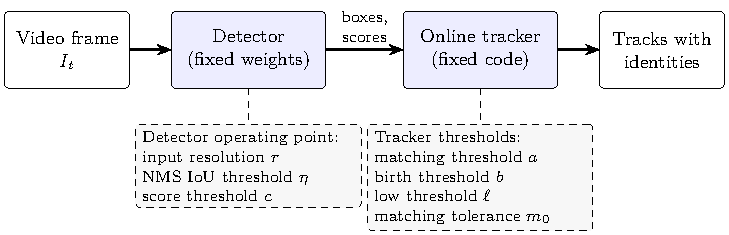
\includegraphics[width=0.95\textwidth]{figures/tbd_pipeline.pdf}
\caption{Tracking-by-detection pipeline and its operating points. The detector settings decide which boxes reach the tracker, and the tracker thresholds decide which of these boxes may match or start a track. In common practice all of these values are fixed for the whole video.}
\label{fig:intro-pipeline}
\end{figure}

This thesis treats these settings as control variables of the tracking system rather than as fixed parameters. It proposes two training-free controllers that adapt them online, from information that is available while the video is processed, with the detector and the tracker left unchanged.

\section{Motivation and Challenges}\label{sec:intro-motivation}
A fixed operating point does not fit a scene that keeps changing. Aerial video makes this especially clear: objects are small, their number changes quickly, the camera moves, and illumination and blur change within one video \cite{zhu2022visdrone,du2018uavdt,cheng2023smallobject}. A setting that works in a sparse, clear scene can keep too much clutter in a dense scene, and a setting that works in a dense scene can lose small or weak objects in another part of the same video. A large input helps small objects, but it costs the same time on easy and hard frames. The choice therefore moves false detections, missed objects, identity switches, and runtime together.

A second problem appears when the detector changes. In real systems the detector is often replaced, retrained, or compressed, while the tracker keeps the thresholds that its authors set for another detector. Detector scores are not calibrated across models and conditions \cite{kuppers2020detcalib}, so a new detector usually gives scores on a different scale, and nothing in the system notices. The effect can be large. ByteTrack in its official setting starts a track only from a box with a score of at least 0.7; if the scores of a published detector are halved, a car that was scored 0.9 now gets 0.45, ByteTrack never starts a track, and its higher order tracking accuracy (HOTA) \cite{luiten2021hota} falls from 67.70 to 0 (Section~\ref{sec:res-shift}).

The main challenges of adapting the operating point in a working system are:
\begin{itemize}
\item \emph{No labels at run time.} A deployed system has no ground truth, so the adaptation must be decided from the video and from the system's own outputs.
\item \emph{Causality and delay.} Only the current and earlier frames may be used, and the extra computation must be small next to the detector, so that the system stays usable in real time.
\item \emph{Unchanged components.} Retraining the detector or rewriting the tracker for every new combination is costly and loses the modularity of tracking by detection; the controller should work from the outside.
\item \emph{Stability.} Each change of the operating point changes the boxes that reach the tracker, so the settings should follow lasting changes of the scene rather than single frames.
\item \emph{No harm when nothing is wrong.} A tracker that already fits its detector should keep its accuracy; an adaptation that always intervenes can lower it.
\end{itemize}

Existing methods address parts of this problem. Adaptive inference methods change the detector configuration, but they usually need an extra learned model and target detection rather than tracking \cite{chin2019adascale,xu2020approxdet,jiang2018chameleon}. Adaptive-threshold methods change thresholds inside one specific tracker \cite{ma2023adaptivebytetrack,shim2024adaptrack,act2026adaptive}, and score calibration methods need labelled data \cite{kuppers2020detcalib}. A simple, training-free way to adapt the operating point of a tracking pipeline online, with the detector and the tracker left unchanged, is missing.

\section{Problem Statement}\label{sec:intro-problem}
Let a video be a sequence of frames $I_1, I_2, \dots$, processed online by a frozen detector and a frozen tracker. The weights of the detector, and the code and association algorithm of the tracker, are not changed. At every frame $t$, a controller may choose only settings that the pipeline already exposes, and it may base its choice only on the current frame, on earlier frames, and on the outputs that the detector and the tracker have already produced. No ground truth, no future frame, and no training is allowed. The goal is to improve tracking accuracy, measured by HOTA, the multiple object tracking accuracy (MOTA), the identity F1 score (IDF1), and the number of identity switches (IDS), while adding little computation.

The thesis studies two forms of this problem:
\begin{enumerate}
\item \emph{Scene-adaptive detector operating point.} In UAV video, choose the confidence threshold, the NMS threshold, and the input resolution of the detector from cheap cues of the scene, so that the boxes passed to the tracker fit the current scene.
\item \emph{Self-calibration to the detector's score scale.} When the detector or its scores change, choose which candidates reach the tracker, the scores they carry, and the tracker's thresholds for the frame, from the scores of recent frames alone, so that a published tracker keeps working with a detector it was not tuned for, and is left as it is when it already fits.
\end{enumerate}

\section{Proposed Solution}\label{sec:intro-solution}
The thesis proposes two rule-based controllers that share the same principles: no learned weights, no labels at run time, use of past information only, unchanged detector and tracker, values fixed before the final evaluation, and paired bootstrap statistics for every comparison. Figure~\ref{fig:intro-outline} shows where they act in the pipeline.

The first controller, Adaptive Control for Multi-Object Tracking (AC-MOT), runs next to the detector. Every ten frames it measures cheap cues of the current image and of the boxes that the tracker reported in the previous frame, averages the recent crowd level into a scene complexity index (SCI), and selects one of three detector operating points through a three-state controller with recovery, hysteresis, and dwell rules. Its thresholds and actions were selected by cross-validation on separate calibration sequences and then frozen.

The second controller, a self-calibrating control layer (SCL), runs once per frame between the detector and the tracker. It splits the score logits of the last ten frames twice with Otsu's method \cite{otsu1979} into background, uncertain, and confident groups, and decides from the share of confident candidates whether the score distribution is clean or noisy. On clean scores it keeps the tracker's scores and thresholds; on noisy scores it chooses the candidates, gives them new scores, and sets the thresholds. A continuation step lets a weak box that clearly continues a track reach single-stage trackers, which have no low-score step of their own. The layer serves different published trackers through four of their published settings, called the host contract.

\begin{figure}[tbp]
\centering
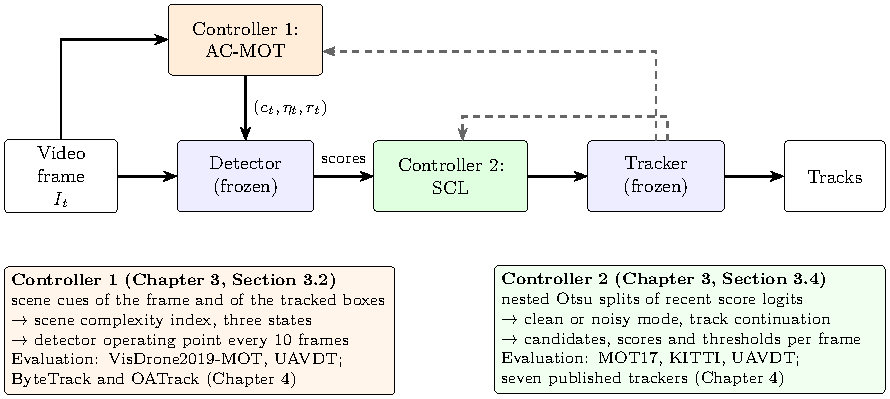
\includegraphics[width=0.98\textwidth]{figures/outline.pdf}
\caption{Outline of the proposed approach. Controller~1 (AC-MOT) sets the detector operating point from scene cues; Controller~2 (SCL) adapts the candidates, scores, and thresholds that the tracker receives from the detector's score distribution. Dashed arrows: tracked boxes of the previous frame.}
\label{fig:intro-outline}
\end{figure}

The contribution of this research is summarized as follows:
\begin{itemize}
\item AC-MOT, a training-free and causal controller that treats the detector operating point as part of the MOT system and adapts it online, with the detector and the tracker unchanged, together with an optimization-guided development path whose final values are selected by cross-validation on calibration sequences.
\item An evaluation of AC-MOT on VisDrone2019-MOT with two trackers, ByteTrack and OATrack, using eight MOT metrics and paired bootstrap intervals, and a transfer to UAVDT without retuning.
\item SCL, a training-free and causal layer that keeps the tracker's scores and thresholds when the scores are clean and takes control only when they are noisy, with a host contract that lets one fixed configuration serve single-stage and two-stage trackers without changing them.
\item An evaluation of one frozen SCL configuration on seven published trackers, four detection sources, and three datasets, including score shifts, predeclared external trackers, a held-out aerial test split, and comparisons with simple adaptive thresholds and the published ACT method.
\item Runtime measurements showing that both controllers add only a few milliseconds per frame.
\end{itemize}

\section{Thesis Organization}\label{sec:intro-organization}
The rest of this thesis is organized as follows.

\textbf{Chapter 2: Background and Literature Review}

This chapter reviews object detection and multi-object tracking, the detectors and trackers used in this work, detector confidence and its calibration, and the related work on adaptive inference, adaptive thresholds, and aerial tracking. It ends with a comparison table of the closest methods and the gap that this thesis addresses.

\textbf{Chapter 3: Proposed Training-Free Adaptive Control Approach}

This chapter presents the two proposed controllers. It describes the scene cues, the scene complexity index, the three-state controller, and the action map of AC-MOT, and how its values were selected; then the score self-calibration, the clean and noisy modes, the track continuation, and the host contract of SCL, and how it was developed and frozen.

\textbf{Chapter 4: Experimental Results and Performance Evaluation}

This chapter describes the datasets, evaluation metrics, and implementation environment, and presents the results of both controllers: AC-MOT on VisDrone2019-MOT and UAVDT, and SCL on MOT17, KITTI, and UAVDT under detector and score changes. It compares the proposed controllers with existing approaches and discusses the results.

\textbf{Chapter 5: Conclusions and Future Work}

This chapter summarizes the findings of the thesis and outlines directions for future work.
